


\tikzset{every picture/.style={line width=0.75pt}} %set default line width to 0.75pt        

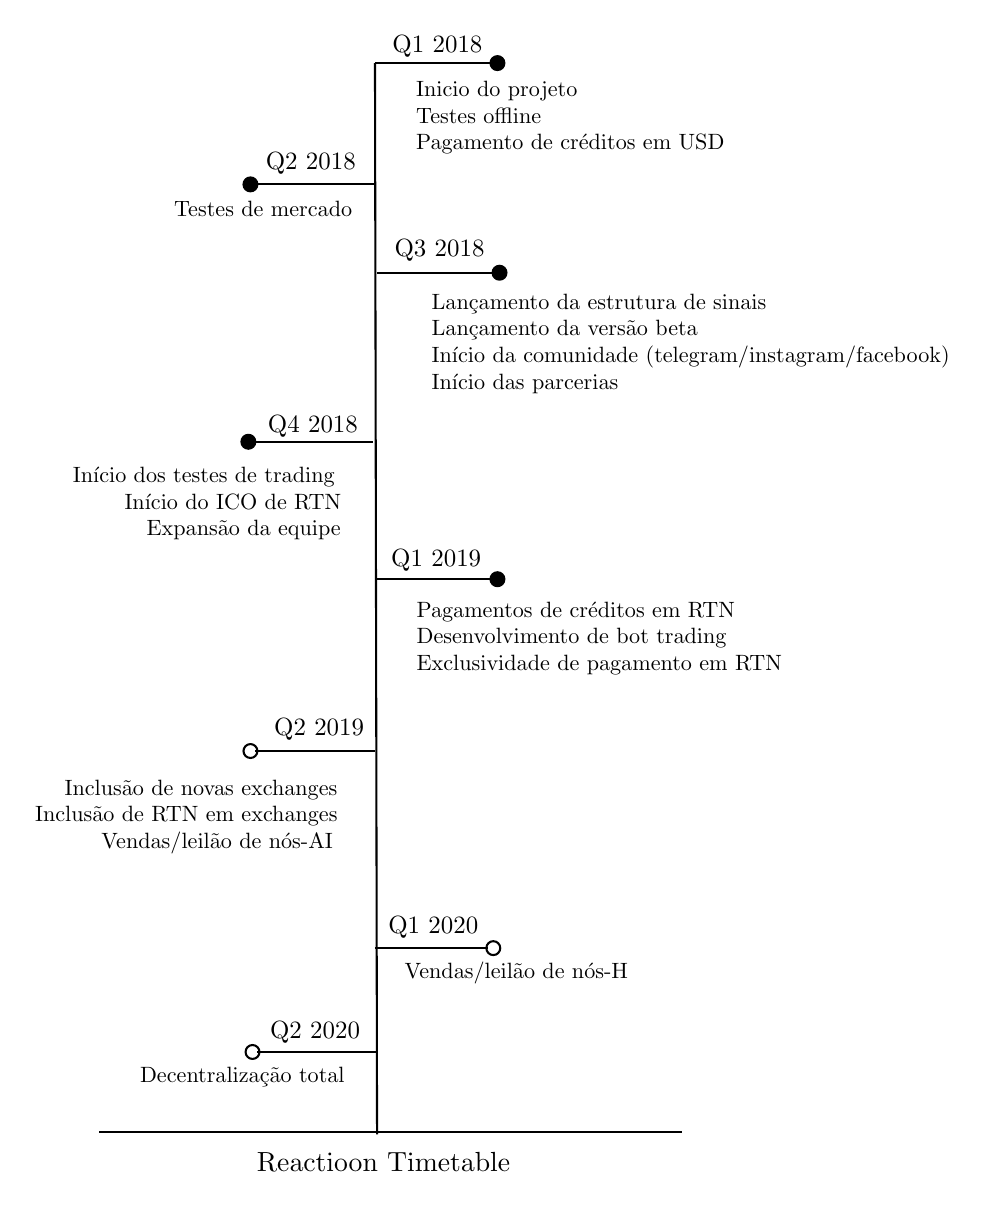
\begin{tikzpicture}[x=0.75pt,y=0.75pt,yscale=-1,xscale=1]
%uncomment if require: \path (0,600.9199981689453); %set diagram left start at 0, and has height of 600.9199981689453

%Straight Lines [id:da27949880366729407] 
\draw    (290.9,47.8) -- (291.9,563.92) ;


%Straight Lines [id:da016695516966388713] 
\draw    (290.9,47.8) -- (349.9,47.8) ;
\draw [shift={(349.9,47.8)}, rotate = 0] [color={rgb, 255:red, 0; green, 0; blue, 0 }  ][fill={rgb, 255:red, 0; green, 0; blue, 0 }  ][line width=0.75]      (0, 0) circle [x radius= 3.35, y radius= 3.35]   ;

%Straight Lines [id:da04938623797133035] 
\draw    (290.9,106.24) -- (230.9,106.24) ;
\draw [shift={(230.9,106.24)}, rotate = 180] [color={rgb, 255:red, 0; green, 0; blue, 0 }  ][fill={rgb, 255:red, 0; green, 0; blue, 0 }  ][line width=0.75]      (0, 0) circle [x radius= 3.35, y radius= 3.35]   ;

%Straight Lines [id:da10792958400592911] 
\draw    (290.9,379.24) -- (233.25,379.24) ;
\draw [shift={(230.9,379.24)}, rotate = 180] [color={rgb, 255:red, 0; green, 0; blue, 0 }  ][line width=0.75]      (0, 0) circle [x radius= 3.35, y radius= 3.35]   ;

%Straight Lines [id:da5389580478447318] 
\draw    (289.9,230.24) -- (229.9,230.24) ;
\draw [shift={(229.9,230.24)}, rotate = 180] [color={rgb, 255:red, 0; green, 0; blue, 0 }  ][fill={rgb, 255:red, 0; green, 0; blue, 0 }  ][line width=0.75]      (0, 0) circle [x radius= 3.35, y radius= 3.35]   ;

%Straight Lines [id:da7641576297357624] 
\draw    (291.9,148.8) -- (350.9,148.8) ;
\draw [shift={(350.9,148.8)}, rotate = 0] [color={rgb, 255:red, 0; green, 0; blue, 0 }  ][fill={rgb, 255:red, 0; green, 0; blue, 0 }  ][line width=0.75]      (0, 0) circle [x radius= 3.35, y radius= 3.35]   ;

%Straight Lines [id:da04724001416544876] 
\draw    (290.9,296.46) -- (349.9,296.46) ;
\draw [shift={(349.9,296.46)}, rotate = 0] [color={rgb, 255:red, 0; green, 0; blue, 0 }  ][fill={rgb, 255:red, 0; green, 0; blue, 0 }  ][line width=0.75]      (0, 0) circle [x radius= 3.35, y radius= 3.35]   ;

%Straight Lines [id:da9347215346833444] 
\draw    (290.9,474.2) -- (345.55,474.2) ;
\draw [shift={(347.9,474.2)}, rotate = 0] [color={rgb, 255:red, 0; green, 0; blue, 0 }  ][line width=0.75]      (0, 0) circle [x radius= 3.35, y radius= 3.35]   ;

%Straight Lines [id:da28779960793088244] 
\draw    (291.9,524.24) -- (234.25,524.24) ;
\draw [shift={(231.9,524.24)}, rotate = 180] [color={rgb, 255:red, 0; green, 0; blue, 0 }  ][line width=0.75]      (0, 0) circle [x radius= 3.35, y radius= 3.35]   ;

%Straight Lines [id:da8846097036360219] 
\draw    (158,563) -- (438.9,563) ;



% Text Node
\draw (385,74.02) node [scale=0.8] [align=left] {Inicio do projeto\\Testes offline\\Pagamento de créditos em USD};
% Text Node
\draw (290,55) node [scale=0.8] [align=left] {};
% Text Node
\draw (237,118) node [scale=0.8] [align=left] {Testes de mercado};
% Text Node
\draw (443,183) node [scale=0.8] [align=left] {Lançamento da estrutura de sinais\\Lançamento da versão beta\\Início da comunidade (telegram/instagram/facebook)\\Início das parcerias};
% Text Node
\draw (321,40) node [scale=0.9] [align=left] {Q1 2018};
% Text Node
\draw (260,96) node [scale=0.9] [align=left] {Q2 2018};
% Text Node
\draw (322,138) node [scale=0.9] [align=left] {Q3 2018};
% Text Node
\draw (261,223) node [scale=0.9] [align=left] {Q4 2018};
% Text Node
\draw (320.4,287.46) node [scale=0.9] [align=left] {Q1 2019};
% Text Node
\draw (264,369) node [scale=0.9] [align=left] {Q2 2019};
% Text Node
\draw (319,464.16) node [scale=0.9] [align=left] {Q1 2020};
% Text Node
\draw (262,515) node [scale=0.9] [align=left] {Q2 2020};
% Text Node
\draw (321,158) node [scale=0.8] [align=left] {};
% Text Node
\draw (210,260) node [scale=0.8] [align=left] {Início dos testes de trading\\ \ \ \ \ \ \ \ Início do ICO de RTN\\ \ \ \ \ \ \ \ \ \ \ Expansão da equipe};
% Text Node
\draw (399,325) node [scale=0.8] [align=left] {Pagamentos de créditos em RTN\\Desenvolvimento de bot trading\\Exclusividade de pagamento em RTN};
% Text Node
\draw (200,411) node [scale=0.8] [align=left] { \ \ \ \ Inclusão de novas exchanges\\Inclusão de RTN em exchanges\\ \ \ \ \ \ \ \ \ \   Vendas/leilão de nós-AI};
% Text Node
\draw (359,486) node [scale=0.8] [align=left] {Vendas/leilão de nós-H};
% Text Node
\draw (227,536) node [scale=0.8] [align=left] {Decentralização total};
% Text Node
\draw (295,577) node  [align=left] {Reactioon Timetable};


\end{tikzpicture}
